\chapter{Konzeption}

Im Kapitel {\em Konzeption} beginnt jetzt die Darstellung der eigenen Arbeit. Dieses Kapitel stellt das Bindeglied zwischen Zielsetzung, Stand der Forschung und der eigentlichen Umsetzung dar. Zusammen mit Implementierung und Evaluation macht die Konzeption den Hauptteil der Arbeit aus.

Typischer Umfang der Konzeption: 5-10 Seiten BA, 15-20 Seiten MA.

\section{WebVR und Learning Managment System (LMS)}
 \subsection{Erstellung eines Unterrichts}
 Die VR Übung ist eine ergänzige Lernmethode für das Lernen. Vor der Durchführung der Übung sollen genügendes Vorwissen angeboten werden. Deswegen wird erst einen Unterricht auf Learning Managment System erstellt.

 Laut der Erklärung im Kapitel Stand der Forschung \glqq Multisensorische und emotionale Wahrnehmungen können die Gedächtnisleitung verstärken\grqq\ sollen die Lernmaterialien des Unterrichts vielfältig sein.  Durch drei Lernmateriallien werden das Vorwissen geboten:
 \begin{enumerate}
    \item Text: Text ist das traditionelle Lernmaterial. Es spielt eine unersetzbare Rolle für Lernen. Die Lesegeschwindigkeit kann der Lernende sich selbst entscheiden. Während des Lesens kann der Leser gut denken, merken und notieren.
    \item Video: Video ist ein intuitives Lernmaterial. Zwei Wahrnehmungen, Sehen und Hören werden aufgerufen, wenn man Video anschaut. Durch Video kann die Handlung sehr konkret gezeigt. Zur Zeit ist Video das beste und verbreitete Medium, praktische Kenntnisse zu vermitteln.
    \item Diagramm: Diagramm ist eine optimale Darstellung für Struktur und Sequenz. Die deutliche visuelle Zeichnungen sind hilfreich für das Verständnis und Gedächtnis.
 \end{enumerate}

 Nach der Sammlung der Vorkenntnisse geht der Lernende durch die Zugang in diesem Unterricht in VR Umgebung rein, und wird die praktische Übung durchgeführt. In der Übung steht das Vorwissen als Hinweise zu Verfügung. Die Hinweise müssen nicht zwingend angeschaut werden, wenn der Lernende die Übung flüssig schaffen kann. Allerdings soll die Hinweise einfach erreichbar sein. Sodass muss der Lernende nicht aus VR Umgebung ausgehen, um Hilfsmittel zu suchen, wenn der Lernende nicht an der Vorkenntnisse erinnern kann. Wenn die Übung geschafft wird, wird der Lernende wieder zu dem Unterricht geleitet.

 Nach der Übung wird ein Test geboten, um das Ergebnis des Lernens zu prüfen. Das Ergebnis des Tests wird in Learning Managment System gespeichert und als Feedback an dem Lehrende geschickt.

 \subsection{WebVR}
 Zwei Ziele des Projekts haben höchste Prioritäten: gute Erreichbarkeit und Verbindung mit LMS.

 Der größte Vorteil der native Apps bei Erreichbarkeit ist offline Benutzbarkeit. Wenn die Applikation installiert ist, muss es während der VR Übung nicht online sein. Allerdings die Installation besitzt viele Kapazität von Rechner oder Smartphone. Wenn viele Übungen werden in eine Applikation eingepackt, führt es zu Missbrauch der Kapazität, weil tatsächlich die geschaffte Übungen nicht gebraucht sind. Wenn jede Übung eigne Applikation hat, wird viele extra Zeit in Installation vor dem Lernen investiert, sodass existiert der Vorteil offline Erreichbarkeit nicht mehr.

 Capterra ist eine Webseite, die deren Benutzer hilft, geeignet Software in unterschiedlichen Bereichen zu finden. Es werden insgesamt 432 Softwares gefunden, wenn \glqq LMS Software \grqq\ gesucht wird. 406 von 432 gefundene LMSs haben web basierte Applikation zu Verfügung. Das heißt, dass 94\% LMS können in Browser laufen lassen.

 WebVR Applikation wird auch in Browser aufgerufen. Ohne software Wechseln wird zu keiner Ablenkung geführt. Außerdem ist die Schnittstelle zwischen Web Applikationen einfach zu implementieren. Darüber hinaus fordert LMS sowieso Internet, kann die Anforderung für Internet von WebVR nicht als Nachteil gelten. 

 Laut oben genannten Gründe wird für WebVR Technik entschieden, die VR Übung zu realisieren.

 \subsection{Verbindung zwischen WebVR Applikation und Learning Managment System}
 Es gibt drei Formen für die Verbindung zwischen WebVR Applikation und Learning Managment System(LMS):
 \begin{enumerate}
   \item WebVR Applikation neben dem Learning Managment System:
     \subitem In LMS wird die Zugang zur VR Umgebung geboten und durch URL können Informationen in VR Umgebung eingefügt werden. In Vr Umgebung wird auch die Zugang zurück zu LMS geboten. Aber keine Information kann von VR Umgebung an LMS übermittelt werden.
     
     Der Vorteil ist, dass die WebVR Applikation unabhängig von LMS ist. Jede LMS kann mit der WebVR Applikation verbinden.
     
     Der Nachteil ist, dass der Umtausch der Informationen ziwischen WebVR Applikation und LMS einspurig ist. Das LMS kann Keine Information von WebVR Appliaktion bekommen. Außerdem wird jede Änderung in WebApp z.B. Umschreibung des Hinweises durch Programmierer gemacht. Der Lehrende ist nicht in der Lage, alleine die Übung zu verbessern oder korrigieren.
     
   \item WebVR Applikation teilweise in dem Learning Managment System:
     \subitem In LMS wird die Zugang zur VR Umgebung geboten, allerdings die Zugang nicht ein URL, sondern erfahrungsmäßig ein Plugin ist. Durch das Plugin kann die WebVR Applikation die versteckte zugängliche Daten der Datenbank des Unterrichts bekommen. Mit solche Daten ist die WebVR Applikation in der Lage, die Daten in Datenbank zu speichern und die Daten aus Datenbank zu lesen. Durch das Middleware wird die gegenseitige Kommunikation zwischen WebVR Applikation und LMS ermöglichen. Obwohl durch URL die zugängliche Daten auch übergetragen werden können, ist es sehr unsicher für das LMS.
     
     Der Vorteil ist, dass die Kommunikation zwischen WebVR Applikation und LMS frei ist. Das heißt, dass die übergetragene Daten nicht nur Parameter sondern auch Bilder, Audios und Videos sein können und das LMS kann die Informationen, die während der Übung in WebVR Applikation erstellt, bekommen. Darüber hinaus kann der Lehrende durch dem Plugin die Inhälte in WebVR Applikation direkt andern.
     
     Die Nachteile sind, dass die WebVR Applikation von dem LMS abhängig ist und die Entwicklung aufwendig ist. Um die Daten barrierefrei überzutragen, muss entsprechende Schnittstelle in WebVR Applikation konfiguriert werden. Bei der Entwicklung werden nicht nur WebVR Applikation, sondern auch das Plugin von LMS geschrieben. Zusätzlich wird eine Datenbank eingerichtet.
     
   \item Learning Management System in WebVR Applikation
     \subitem Bei dieser Form ist die Methode der Kommunikation zwischen WebVR Applikation und LMS gleich wie die zweite Form. Der größte Unterschied liegt an der Benutzererfahrung. Die Graphical User Interface(GUI) des LMSs wird in der VR Umgebung dargestellt. Das heißt, dass vom Anfang an der Lernende in der VR Umgebung steht. In der VR Umgebung wird Vorwissen gesammelt, praktische Übung durchgeführt und Test gemacht.
     
     Der Vorteil ist, dass der ganze Lernprozess in VR Umgebung integriert wird, keine Ablenkung existiert.
     
     Die Nachteile sind aufwendige Entwicklung und ungewöhnliche Erfahrung des Lesens.
 \end{enumerate}
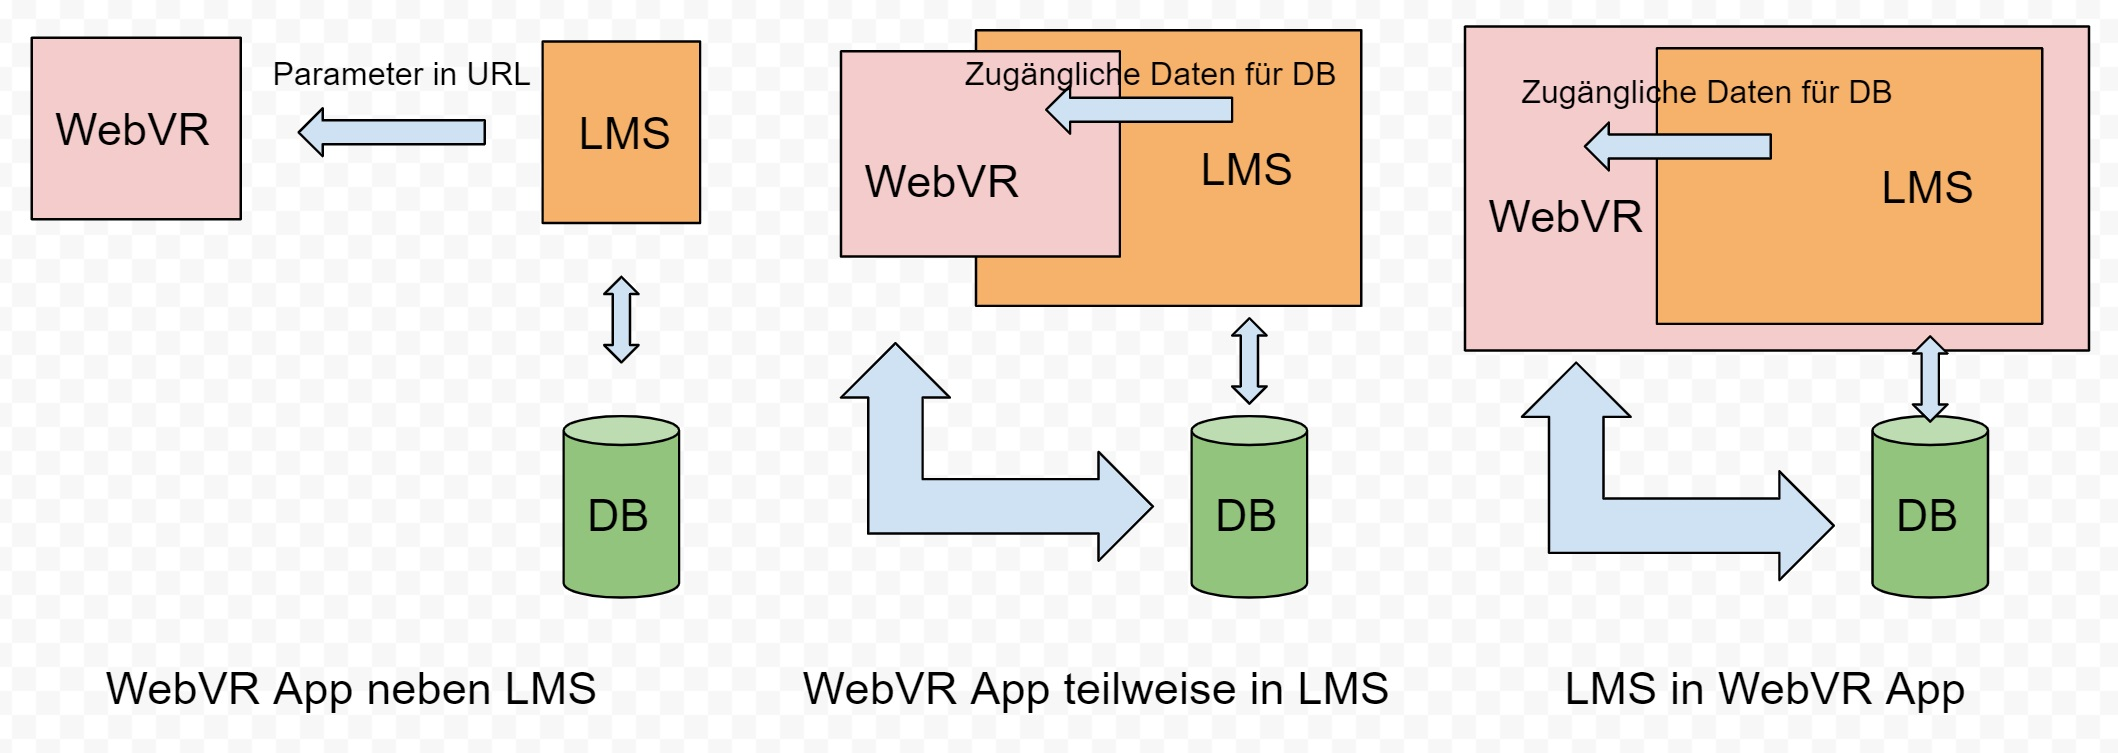
\includegraphics[width=\textwidth]{images/formenDerVerbindung.jpg}

Bei diesem Projekt wird erste Form implementiert. Wegen der begrenzte Entwicklungszeit werden die zweite und dritte Formen bei diesem Projekt nicht realisiert.

\section{Vorbereitung einer Infusions mit WebVR}

 \subsection{GUI}
  \subsubsection{Szene}

  \subsubsection{Hand}
  
  \subsubsection{Durchsichtlichkeit}

 \subsection{Interaktion}
 Interaktion ist der Hauptteil der WebVR Applikation, weil die nicht nur die Implementierung von Interactability von der Kategorie der Immersion ist, sonder auch enge Beziehung mit Matching hat.\citep{28} Da die WebVr Applikation cross-platform ist, werden die Konzeptionen der Interaktion nach den Typen der Geräte gliedert.

 Für jede Geräte wird von drei Aspekten die Interaktionen erklärt:

 \begin{enumerate}
    \item \textbf{Exploration}: Änderung der Aspekt.
    \item \textbf{Navigation}: Translation der Kamera.
    \item \textbf{Manipulation}: Aktivierung der Aktivität des Objektes für PC, Smartphone und Samsung Gear VR, zusätzlich Überprüfung, Greifen und Befreiung für HTC Vive.
 \end{enumerate}

 \subsubsection{Desktop und Laptop}
 text.......................
 
  \textbf{Exploration}
  
  Um die VR Umgebung zu explorieren, wird den Aspekt verändert. Der Aspekt ist die Sicht, die in Kamera aufgenommen ist, nämlich die Sicht des Benutzers. Die Bewegung des Aspekts wird nach der Bewegung der Maus geführt. Es gibt zwei Varianten, um die Bewegung des Aspekts zu bestimmen.
  
  Eine Variante ist, dass die Bewegung des Aspekts aufgerufen wird, wenn die linke Taste der Maus gedrückt. Wenn die linke Taste losgelassen wird, bewegt sich der Aspekt nicht. Der Vorteil ist, dass solche Interaktion ähnlich wie alltägliche Applikation beispielsweise Google Map. Sodass wird die Interaktion schnell gewöhnt. Der Nachteil ist, dass eine Aktivität durch zwei Aktionen, Maus Druck und Maus Bewegung, aufgerufen werden. Das macht die Interaktion kompliziert, wenn der Aspekt sich häufig bewegt.
  
  Die andere Variante ist, dass die Bewegung Mode aktiviert wird. Das heißt, dass die Aspekt sich solange nach der Maus bewegt, bis ESC Taste gedrückt wird. Der Vorteil ist, dass die Interaktion einfach ist, und der Druck auf Maus verringert wird. Der Nachteil ist, dass der Mauszeiger während der Bewegung Mode verschwindet ist. Es könnte passiert, dass der Benutzer die Maus in einer großen Auswahl schwenkt, um den Mauszeiger zu finden, sodass der Aspekt auch schwer wackelt.
  
  Die verwirrende Aktivität bei zweite Variante passiert normalerweise nur bei der erst mal Nutzung und ist harmlos. Allerdings der Vorteil davon ist eindeutig. Deshalb wird die zweite Variante implementiert.
  
  \textbf{Navigation}
  
  Die Position der Kamera ist der Ort, wo der Benutzer in der VR Umgebung steht. Die Trandslation der Kamera führt zu die Navigation des Benutzers in dem simulierten Raum. Zwei Möglichkeiten der Navigation werden gebogen, eine zwingende und eine freiwillige.
  
  Zwingende Navigation bedeutet, dass die Kamera sich automatisch zu einem Ort bewegt, wenn die Translation die Benutzererfahrung verbessern kann. Das Ziel ist, der Benutzer zu leiten, Objekten zu betrachten. Zum Beispiel soll die Plakate über die Desinfektion der Hände Während der Desinfektion richtig betrachtet werden, deswegen bewegt sich die Kamera zwingend zu der Plakate, wenn der Benutzer Hände desinfizieren will.

  Außer der zwingende Bewegung kann die Kamera durch dem Druck auf den Tasten W, A, S, D navigieren. Das bietet die Freiheit, die VR Umgebung sich umzuschauen. Ohne die freiwillige Navigation kann die Übung auch barrierefrei durchgeführt werden.
  
  \textbf{Manipulation} 
  Die Manipulation wird durch dem Zeiger durchgeführt. Zeiger ist ein schwarzer Ring, der immer in der Mittel der Sicht der Kamera steht. Der ist zuständig für den Aufruf eine Aktivität eines Objekts.
  
  Wenn der Benutzer mit dem nächsten Objekt hinter dem Zeiger interagieren kann, wechselt der Farbe des Rings zu grün, um das Selbstvertrauen dem Benutzer zu geben, die Aktivität zu aktivieren. Allerdings bedeutet der grüne Zeiger nicht, dass die Aktivität des Objekts aktiviert werden darf. Die Übung wird nach einer bestimmtem Reihenfolge durchgeführt, wenn eine Aktivität noch nicht daran ist, darf sie nicht aktiviert werden.
  
  Wenn der Zeiger grün ist und die linke Taste der Maus gedrückt wird, scheint die Farbe des Zeigers rot für ca. 0,3 Sekunde, und ein kurzes Soundeffekt geklungen wird, um die Botschaft an dem Benutzer geben, dass der Befehl, mit einem Objekt zu interagieren, ausgeführt ist. 
  
 \subsubsection{Smartphone}
 text.....................
 
  \textbf{Exploration}
  
  Zwei Methoden werden für Exploration angeboten, um unterschiedliche Situation anzupassen.
  
  Die intuitive Methode ist, das Smartphone zu bewegen. Der simulierte Umgebung wird in Smartphone räumlich dargestellt. Aber wegen die Begrenzung des Bildschirms ist nur den Raum teilweise im Blickwinkel. Durch die Bewegung des Smartphones wird andre Ort in dem Raum gesehen.
  
  image: Aspekt smartphone..........................
  
  Es ist unvermeidbar, den Körper zu drehen, um seitig gelegte Objekt zuzuschauen, wenn man mit der erste Methode das Smartphone bewegt. Allerdings ist es unmöglich, großer Winkel zu drehen, wenn man auf einem Stuhl sitzt. Außerdem beeinflusst es anderen Leute, wenn man in öffentlichem Raum beispielsweise Bibliothek große Bewegung macht. Um die Probleme zu lösen, wird die zweite Methode angeboten, dass der Aspekt durch dem Ziehen auf Bildschirm verändert wird. Obwohl diese Methode nicht so intuitive wie die erste Methode ist , vermehrt es sich die Einsatzmöglichkeiten.
  
  \textbf{Navigation}
  
  Das Smartphone bietet nur 3DoF Erkennung, nämlich Rotation. Deswegen kann die Translation des Kamera nicht mit der Translation des Smartphones verbinden. Um Objekt genauer anzuschauen und Interaktion zu vereinfacht, wird zwingend Navigation wie auf Laptop angeboten.
  
  \textbf{Manipulation}
  
  Der Form des Zeigers ist gleich wie auf Laptop. Da keine Maus zu Verfügung für Smartphone ist, wird die Bestätigung aus Zeiger durch \glqq Anstarr\grqq\ (eng. gaze) gesendet. Wenn der Zeiger vor einem Objekt ca. 0,5 Sekunde beliebt ist, wird es versucht, die Aktivität des Objeckts durchzuführen. Gleichzeitig wird ein kurz Soundeffekt geklungen.
  
 \subsubsection{Samsung Gear VR}
 Samsung Gear Vr ist ein Beispiel für das 3Dof HMD. Gear VR kann mit oder ohne Controller benutzt werden.
  \textbf{Exploration}
  
  Durch Gear VR wird der Benutzer in dem simulierten virtuellen Raum eingesetzt. Die Exploration wird durch der Rotation des Kopfs durchgeführt, ähnlich wie in reales Leben. Allerdings wird nur Rotation von HMD erkannt, weil Gear VR 3DoF ist.
  
  \textbf{Navigation}
  \begin{itemize}
  \item \textbf{Ohne Controller}: Wenn Gear VR ohne Controller ist, kann es Google Cupboard gelten. Die Navigation ist gleich wie die Navigation mit Smartphone, dass nur zwingend Navigation angeboten ist.
  \item \textbf{Mit Controller}: Der Gear VR Controller ist ein 3DoF Controller, dass nur die Rotation erkannt wird. Es soll eine Kurve aus dem Controller ausstrahlen, die auf dem Boden landen soll. Dort wird als der Zielort gezeichnet. Wenn den Tranlation Befehl durch dem Druck auf dem Trackpad auf dem Gear VR Controller gesendet, soll die Kamera sich zu dem gezeichnete Position navigiert.
  \end{itemize}
  
  \textbf{Manipulation}
  \begin{itemize}
  \item \textbf{Ohne Controller}: Der Zeiger kann in zwei Formen möglich sein.
  
  Eine Möglichkeit ist, dass der Zeiger gleich wie auf Laptop und Smartphone als Ring gezeigt. Der Vorteil ist, dass der Zeiger eindeutig ist. Der Ring ist auf dem komplizierten Hintergrund (die Objekten in dem Raum) einfach zu kennen. Der Nachteil ist, dass der Treffpunkt mit Objekte nicht klar ist , besonders wenn das Ziel klein ist.
  
  Die andere Variante ist durch Raycaster. Raycaster ist eine von einer bestimmten Position ausstrahlende Linie, die die durchgegangene Objekte erkennen kann. In diesem Projekt wird das nächste Objekt zu dem Ausgangspunkt der Linie als das getroffene Objekt gezeichnet. Ein aus Augen Position ausstrahlendes Raycaster kann als der Zeiger gelten. Der Vorteil ist, dass die Position des Treffpunkts ganz genau ist. Der Nachteil ist, dass die Linie vor dem Komplizierten Hintergrund nicht auffallend ist.
  
  Die Merkmale der beiden Varianten sind eindeutig. Die Entscheidung für wird bei der Implementierung nach dem Endeffekt treffen.
  
  Die Bestätigung aus Zeiger kann durch dem Druck auf Touchpad von Gear VR oder auch durch \glqq Anstarr\grqq\ wie auf Smartphone durchgeführt werden. Als Feedback der Bestätigung wird ein kurz Soundeffekt geklungen. 
  
  \item \textbf{Mit Controller}: Ein Raycaster soll aus dem Controller ausstrahlen. Durch einem Druck auf dem Auslöser auf dem Controller wird es versucht, die Aktivität des getroffenen Objekt zu aktivieren. 
  \end{itemize}
  
  image: controller Gear VR....................
  
 \subsubsection{HTC Vive}
 HTC Vive ist ein Beispiel für das 6DoF HMD.
 
  \textbf{Exploration}
  
  Gleich wie mit Gear VR wird die Bewegung des Aspekts auch durch der Bewegung des Kopfs durchgeführt. Da HTC Vive 6DoF ist, werden nicht nur die Rotation sondern auch die Translation  erkannt. Sodass ist HTC Vive in der Lage, die Bewegung des Kopfs in der VR Umgebung völlig zu simulieren.
  
  \textbf{Navigation}
  
  Auch gleich wie mit Gear VR strahlt eine Kurve aus dem Controller, die auf dem Boden landet, und den Zielort zu bezeichnen. Durch dem Druck auf dem Trackpad auf dem Controller wird die Bewegung bestätigt und durchgeführt.
  
  \textbf{Manipulation}
  \begin{itemize}
  \item \textbf{Aktivierung der Aktivität des Objektes}: Durch dem Druck auf dem Auslöser wird es versucht, die Aktivität des Objektes zu aktivieren.
  \item \textbf{Greifen}: Wenn der Controller mit einem Objekt überlappt und der Auslöser auf dem Controller gedrückt und nicht befreit wird, wird das Objekt in dem Hand(Controller) gegriffen.
  \item \textbf{Befreiung}: Wenn ein Objekt in einem Hand(Controller) ist und deren Auslöser losgelöst wird, wird das Objekt befreit. Das heißt, dass das Objekt entweder auf eine bestimmte Position gelegt wird oder fällt.
  \item \textbf{Überprüfung}: Wenn ein Objekt überprüft werden muss, wird ein Raycaster aus der Position der Augen ausstrahlt. Wenn das Raycaster die richtige Position trifft und der Auslöser von einem leeren Hand gedrückt wird, wird die Überprüfung durchgeführt.
  \end{itemize}
  
 \subsection{Anordnung}
  \subsubsection{Ablauf}
  
  \subsubsection{Abschnitte}
  
  \subsubsection{White board}
  
  \subsubsection{Hacken}
  
  \subsubsection{Hilfe Boxes}
  
\begin{itemize}
\item UI
\item white board
\item Interaktion
\subitem flach Bildschirm: cursor, gaze
\subitem GearVR: gaze, click
\subitem HTC Vive: drag, press release, hand, check
\subitem observer patern---------
\item Töne
\item section selection: observerpatern------
\item hand
\item collision
\item check 3 Dingen
\end{itemize}